% INTERCEPT 2027 submission, Defenders track. IEEE conference
% template (Overleaf "IEEE Conference Template", IEEEtran). Blind
% review: no author name, organization, or repository link anywhere
% in this file. Prose follows paper/INTERCEPT_DRAFT.md (the master);
% every number is on the ledger in paper/FREEZE_2026-09-26.md.
\documentclass[conference]{IEEEtran}
\IEEEoverridecommandlockouts

\usepackage{cite}
\usepackage{amsmath,amssymb,amsfonts}
\usepackage{graphicx}
\usepackage{booktabs}
\usepackage{textcomp}
\usepackage{xcolor}
\usepackage[hidelinks]{hyperref}

\graphicspath{{figures/}}

\newcommand{\rows}{\textsuperscript{$\dagger$}}
\newcommand{\tvd}{\mathrm{TVD}}

\begin{document}

\title{Judgment-Layer Drift, No Changelog:\\
56 Days Monitoring Five LLM APIs}

\author{\IEEEauthorblockN{Blind submission}
\IEEEauthorblockA{Defenders track}}

\maketitle

\begin{abstract}
Served LLM behavior changes behind stable model ids, and the change
has a shape. I ran a calibrated behavioral monitor against five
production LLM APIs daily for 56 days: a frozen 68-item security
judgment bank, $K{=}10$ samples per item, per-item total variation
distance against a frozen baseline, simulation-calibrated alarm
bands, and a same-day disambiguation rerun on every breach. Three
findings. First, judgment behavior oscillates rather than drifts.
Models revisit exact prior answer distributions on contested items:
one item returned to the identical unanimous vector on four of its
five breach days, another to the identical 8/0/2/0 split on five of
seven, and entries arrive as same-day joint moves across items.
Dwell runs from one daily observation to weeks. Second, the movement
concentrates entirely where judgment is contested. All 75 breach
entries landed on designed-equipoise items; the 225 decisive slots
produced zero breaches in 11,057 slot-days; and quiet equipoise
slots on every vendor moved no more than exact sampling arithmetic
predicts. The breach count itself is not evidence, and I say so: 75
sits below the 92 a conservative null expects. The structure is the
evidence. Thirteen slots carry three or more entries against 1.04
expected ($P = 6.7\times10^{-11}$), and ten of the thirteen moved
toward the same option every time. Third, every serving covariate
visible from outside held constant across 174,033 rows while
behavior moved, until the one covariate that did move was the
identity string itself: one vendor silently aliased the pinned id
mid-study, and only the response-side echo caught it. A customer
can detect the change and cannot attribute it. A snapshot
evaluation certifies the day it ran, not the period it is cited
for. The monitor costs about 20 USD per month, and the instrument,
the record, the analysis, and every correction are reproducible
from a public artifact.
\end{abstract}

\begin{IEEEkeywords}
LLM API monitoring, behavioral drift, runtime security, agent
assurance, change detection, false-alarm calibration
\end{IEEEkeywords}

\section{Introduction}

An agent pipeline is qualified against the model serving it.
Nothing announces when that stops being true. Vendors change
weights, quantization, serving configuration, and safety layers
behind stable model ids; the response schema carries no version for
any of it. A control validated last quarter is not validated today,
and no signal reports the expiration.

The gap is not hypothetical. One vendor's published postmortem
documents three concurrent serving-stack bugs, sticky per-user,
missed by the vendor's own evaluations and resolved by
rollback~\cite{anthropic-postmortem}. That is the vendor telling us
what the serving layer does when nobody is measuring from outside.

Here is what measuring from outside looks like. On August 2, 2026,
I baselined five production APIs on a 68-item judgment bank and
probed the full bank hours later: 340 slots, zero breaches, every
model clean. The next scheduled probe, one day later, found one
model in a different regime: two items flipped to a joint state
they had occupied four days before, at probabilities on the order
of $10^{-4}$ to $10^{-14}$ under the fresh baseline. The state held
for the same-day rerun, reverted days later, and returned again.
This is not an outage and it is not noise. It is a served model
revisiting a prior behavioral state, on a pinned id, with no
changelog entry. Fifty-six days later the record holds 75 such
entries on 17 slots, and not one on a decisive item.

This paper contributes:
\begin{enumerate}
\item[(a)] the first documentation, to my knowledge, of reversible
  day-scale regime oscillation in served LLM judgment behavior,
  with exact recurrence of prior answer distributions;
\item[(b)] a drift instrument built from a stratified judgment
  bank, designed-equipoise items alongside decisive ones, with an
  11,057 slot-day zero-breach null on the decisive class;
\item[(c)] detection-without-attribution measured jointly: behavior
  moved while every observable covariate held, and the one
  covariate that moved carried no explanation either;
\item[(d)] per-vendor temporal phenotypes on two axes, per-call
  commitment and drift morphology: quiet slots show no excess
  movement on any of the five models, and drift, where it occurs,
  is discrete unidirectional oscillation on four vendors and
  mixed-direction wander on one;
\item[(e)] the instrument itself: reproducible, vendor-agnostic,
  roughly 20 USD per month to operate, with 56 days of
  pre-registered decision rules, corrections, and one full
  re-baseline loop in its public history.
\end{enumerate}

\section{Instrument}

The bank is 68 forced-choice enterprise security judgment items,
four options each: 45 decisive items with a derivable best answer
and 23 designed-equipoise items authored to sit near a decision
boundary. Five production models, one pinned arm each, $K{=}10$
samples per item, daily at 13:00 UTC. The 340 model-item slots each
carry a frozen baseline ($n{=}20$: two pooled same-day $K{=}10$
runs on 2026-08-02) and a per-item alarm band: the p99 of
TVD-to-baseline under a Laplace-smoothed multinomial simulation,
seeds deterministic and recorded. Bands across the 340 slots: 0.40
on 311 slots, 0.45 on 28, 0.50 on 1 (Table~\ref{tab:t2}).

A day's probe compares each slot's observed distribution to its
baseline. A breach (strict inequality above band) fires a same-day
rerun of the breached items only, and the rerun disambiguates: a
rerun matching the probe and not the baseline is an EVENT, matching
the baseline back is TRANSIENT, matching neither is UNSTABLE. Every
response row records the echoed model id; a divergent echo halts
collection for that model at the first call (ECHO\_CHANGE,
exercised from day 40 of the record onward; Section~\ref{sec:attr}).
One verdict line per model per day, appended to a committed log.
The verdict grammar is CLEAN, EVENT, TRANSIENT, UNSTABLE,
ECHO\_CHANGE, ERROR, and the reporting commitment was declared
before the first scheduled observation: quiet windows get published
with the same care as event windows.

The false-alarm rate is not assumed from the band percentile. It is
computed by exact enumeration over all 286 compositions of ten
draws into four options, per item, against each item's band: 1.65
expected false breaches per day if the smoothed baseline is truth,
0.05 if the empirical baseline is truth. Observed daily breach
counts sit against that null throughout. The comparison is a strict
inequality implemented in floating point, and Section~\ref{sec:wrong}
reports what that decided.

The record at the freeze is 56 calendar days, 2026-08-02 to
2026-09-26, with 166,006 calls in the verdict log and at least one
probe on 55 of the days. Availability gaps, all recorded in the log
and none a behavioral observation: one vendor arm lost three days
to account credit exhaustion (HTTP 429), the two arms on a second
vendor lost two days to a credential rotation on my side (HTTP
401), a third vendor's arm returned HTTP 503 ``high demand'' on ten
days including the eight ending at the freeze, and one day failed
on all five arms from a local network outage. A fifth arm halted
itself on day 40 and stayed halted (Section~\ref{sec:attr}).
Everything above is regenerable from the committed repository:
baselines, bands, seeds, verdict log, derived daily counts, and
every analysis script behind a number in this paper. Numbers marked
\rows{} come from the raw per-call rows, which embed full model
replies and are retained by the operator rather than published.

\begin{table}[t]
\caption{Instrument summary.}
\label{tab:t2}
\centering
\small
\begin{tabular}{@{}p{0.30\columnwidth}p{0.62\columnwidth}@{}}
\toprule
parameter & value \\
\midrule
item bank & 68 forced-choice judgment items (45 decisive, 23 designed-equipoise) \\
models & 5 production APIs, one pinned arm each \\
alarm slots & 340 (115 equipoise), zero sentinels \\
cadence & daily, 13:00 UTC, $K{=}10$ samples per item \\
baseline & frozen $n{=}20$ per slot (two pooled same-day $K{=}10$ runs, 2026-08-02) \\
alarm bands (p99) & 0.40 on 311 slots, 0.45 on 28, 0.50 on 1 \\
breach test & per-item TVD vs baseline, strictly above band; same-day rerun disambiguates \\
verdict grammar & CLEAN, EVENT, TRANSIENT, UNSTABLE, ECHO\_CHANGE, ERROR \\
expected false breaches & 1.65/day (smoothed truth), 0.05/day (empirical truth), exact enumeration \\
record at freeze & 56 probe days, 166,006 calls \\
operating cost & about 20 USD per month \\
\bottomrule
\end{tabular}
\end{table}

\section{Findings}

\subsection{Regime oscillation with exact recurrence}
\label{sec:osc}

The headline behavior is not drift in the gradual sense. It is
discrete states, revisited exactly (Fig.~\ref{fig:f1},
Fig.~\ref{fig:f2}).

One vendor's model held a two-item joint state (unanimous terse A
on a fraud-scoring item; verbose 9 or 10 of 10 D on a
vulnerability-gating item), left it, and re-entered it three days
later, with both items breaching together on three of the five
breach days and exits staggering across days. The fraud-scoring
item produced the identical pure-A vector, 10/0/0/0, on four of its
five breach days (Aug 3, 4, 6, 10). A second vendor's offboarding
item produced the identical 8/0/2/0 on five of its seven breach
days. A third vendor's spend-anomaly item produced the identical
0/6/0/4 on seven of its ten. These are the vectors on which the
alarms fired; the same items also sat away from baseline inside
band on many more days, at vectors that recur too (the offboarding
item at 6/0/4/0 and 7/0/3/0 five days each).

Under the frozen baselines these are not plausible draws. The
recurring pure-A state has per-run probability $1.0\times10^{-4}$
under the empirical baseline and $5.5\times10^{-5}$ under the
smoothed one; the 0/0/0/10 verbose state on the vulnerability item,
$1.6\times10^{-14}$ smoothed and zero empirical; the 0/6/0/4 state,
$1.7\times10^{-6}$ empirical. The states are also not new: they are
prior observed states of the same items. That is what motivates
calling this oscillation rather than drift. Dwell in a state runs
from one daily observation (the two gpt items with unanimous
baselines never held an excursion past a single day in 52 observed)
to weeks (Section~\ref{sec:loop}). The same-day rerun bounds
within-state persistence from below: across the record the gap
from the last probe sample of a breached item to its first rerun
sample runs 0.34 to 10.15 minutes, median 1.86\rows, and the rerun
reproduced the probe vector exactly on 8 of the 75 entries.

\begin{figure*}[t]
\centering
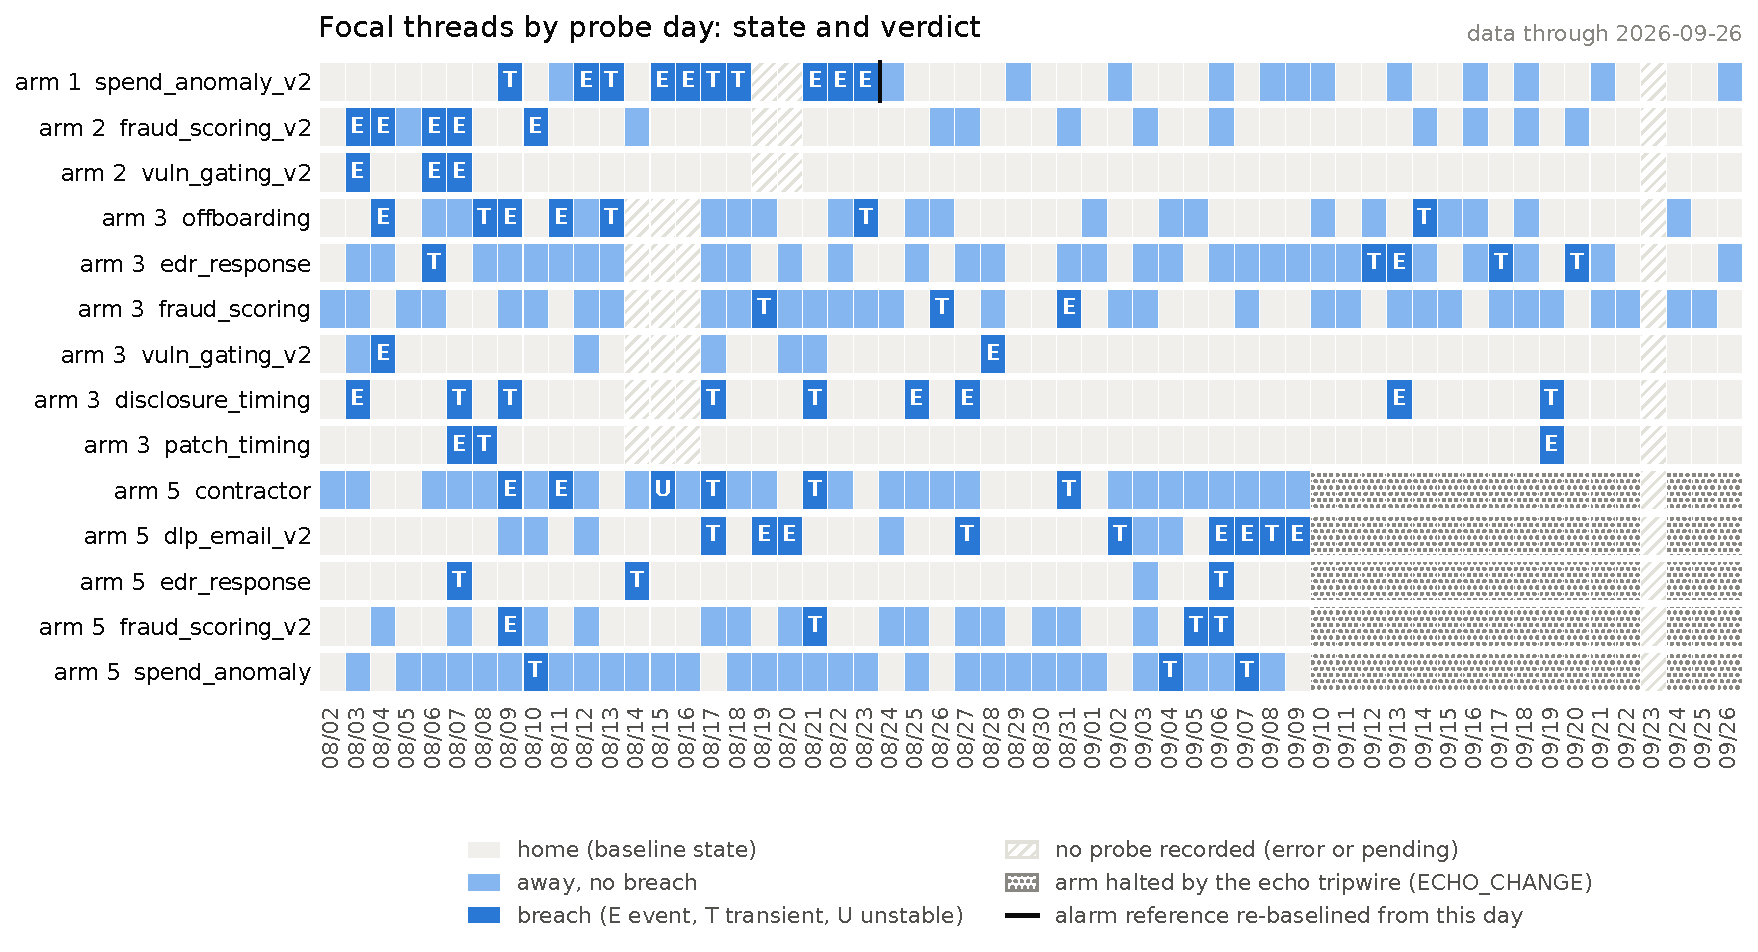
\includegraphics[width=\textwidth]{f1_regime_map.pdf}
\caption{Regime map. Fifteen focal threads (every model-item slot
with two or more breach entries) by probe day. Light cells are
home (no breach, baseline modal), mid-blue cells are away without a
breach, dark cells are breaches with their verdict letter, hatched
cells are days with no probe, dotted cells are days the echo
tripwire halted the arm, and the dark edge on the first row marks
the day that slot's alarm reference was re-baselined. Data through
2026-09-26.}
\label{fig:f1}
\end{figure*}

\begin{figure*}[t]
\centering
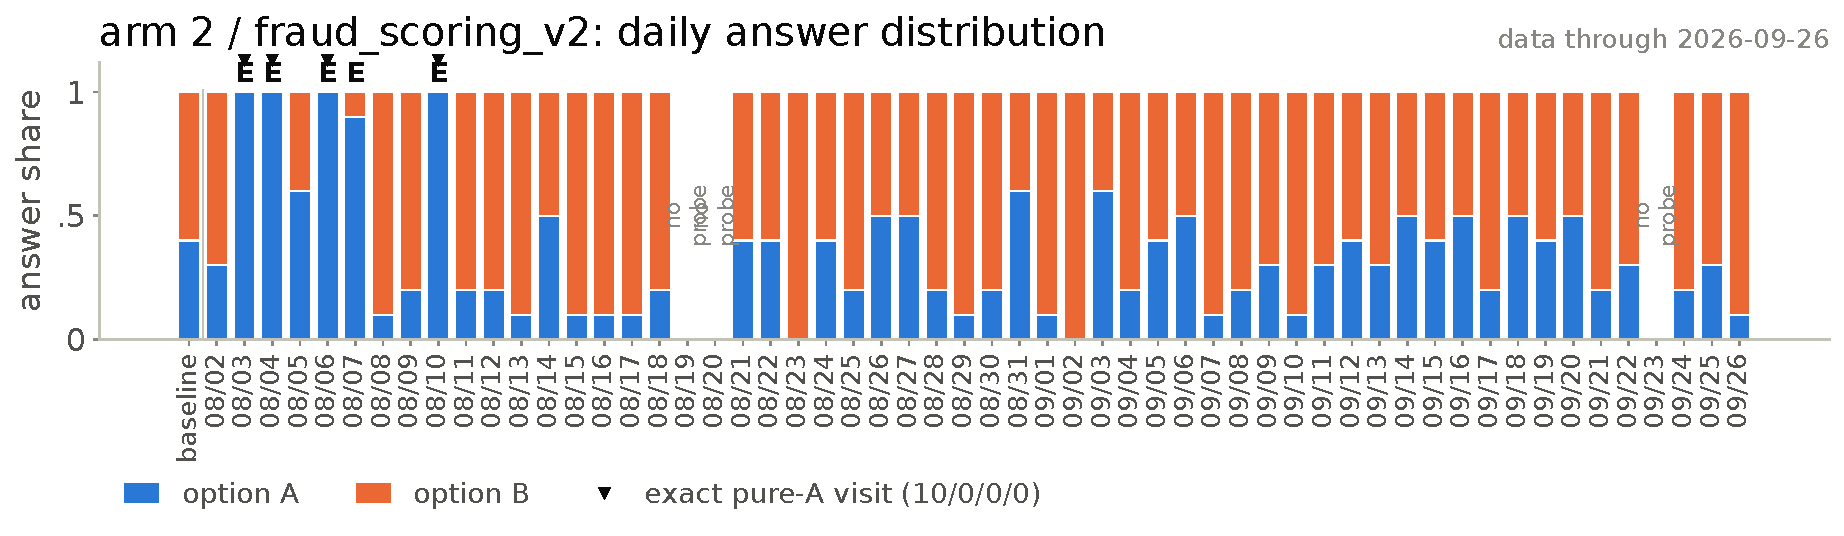
\includegraphics[width=\textwidth]{f2_recurrence_strip.pdf}
\caption{Exact recurrence. Daily answer distribution of the
fraud-scoring item on the sonnet arm, with the frozen pooled
baseline at left. Markers above the bars are the four identical
pure-A visits; letters are verdict-log breaches. The item alternates
between a split state near its baseline and an exact unanimous
state it re-enters.}
\label{fig:f2}
\end{figure*}

\subsection{The pre-committed step-change rule, and one full loop}
\label{sec:loop}

The rule, committed 2026-08-16 blind to the deciding data, resolved
the first episode on the haiku spend-anomaly item as alternation on
its first evaluated day (a home visit on Aug 14). A second away run
began Aug 15 and crossed the pre-committed threshold on 2026-08-23:
seven consecutive observed away days, and the rule designated the
item a step-change candidate with no judgment in the loop. The
operator response was a dual-reference re-baseline: the alarm
reference moved to the new state, the frozen original stayed
preserved in the same record, and a return criterion against the
original was pre-registered before any new-regime data accrued. The
criterion fired on post-rebaseline day 10. On 2026-09-02, after
sixteen consecutive observed away days spanning the re-baseline,
the item revisited the original reference: inside the superseded
band, modal restored, on a vector identical to two of its early
home-dwell days four weeks prior. The pre-registered branch
executed the same day as a dated commit. The classification was
revised to slow alternation with week-scale dwell, the candidacy
stands as a correctly fired rule, and the re-baseline was
re-examined as pre-committed and kept: the item rests in the new
state and visits the old one, and the preserved original is what
made the return visible at all. After the revision the item visited
the original reference on seven days through Sep 18 and then sat
away for the seven observed days ending at the freeze. Against the
frozen reference it was home on 16 of 53 observed days. This was
not a step change. It is the longest-dwell alternation in the
record, and every step of the loop, rule, candidacy, re-baseline,
return criterion, revision, ran on machinery pinned before its
deciding data existed.

Four more rules were pinned on other threads as their away runs
lengthened (thresholds of 12, 8, 3, and 4 consecutive observed away
days, each derived from the thread's own longest returned-from
dwell plus two days of clearance). None fired. The longest count
any reached was 4 of 12. A fifth, on the deepseek data-loss item,
stood at 2 of 5 when the arm's identity changed and is suspended,
not resolved. Two of the five pins carry a registration caveat in
the record (one was merged after post-pin data existed, and its
blindness rests on attestation; two sessions drafted one rule under
the same filename and the collision is documented); I report the
grades rather than hide them.

\subsection{The movement concentrates where judgment is contested}
\label{sec:conc}

Every breach the monitor recorded is an equipoise item. All 75
breach entries across 56 days landed on designed-equipoise slots,
on 17 distinct slots; the decisive class produced zero breaches in
11,057 slot-day observations. The honest null share for the
equipoise class is 0.383 of breach mass (not the 0.338 uniform
share; equipoise bands sit differently), and the concentration
survives that weighting: $P(\text{all 75 entries on equipoise}) =
5.1\times10^{-32}$, $P(\text{all 17 distinct slots on equipoise}) =
8.1\times10^{-8}$.

The claim needs its ceiling stated. At $K{=}10$ the bands sit near
TVD 0.4 regardless of item distribution, so a breach on a unanimous
baseline needs five of ten samples to change category, and four on
a mixed one. Decisive items sit unanimous at baseline; registering
movement there requires close to an outright answer flip. Decisive
silence is an instrument ceiling, not demonstrated stability. What
the decisive record does show is how little they move at all: the
maximum decisive slot-day TVD in 11,057 was 0.30, reached twice;
seven slot-days exceeded 0.20 (Fig.~\ref{fig:f3}). The defensible
claim is that detectable movement lives on contested judgment, and
clear-cut behavior stayed frozen at the resolution this instrument
has.

\begin{figure}[t]
\centering
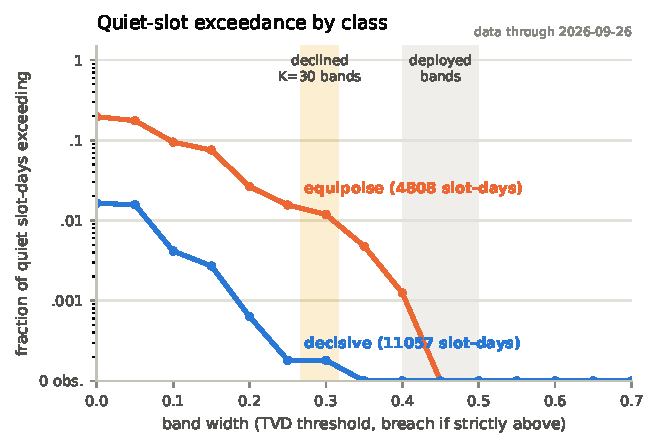
\includegraphics[width=\columnwidth]{f3_false_alarm_curve.pdf}
\caption{Quiet-slot exceedance by class. Fraction of slot-days on
never-breached slots whose TVD to baseline strictly exceeds each
candidate band width, on the $K{=}10$ lattice. The deployed bands
(0.40 to 0.50) and the declined $K{=}30$ bands (0.267 to 0.317) are
shaded. Decisive slot-days never exceed 0.30; equipoise slot-days
exceed the declined bands at 0.7 to 1.5 percent.}
\label{fig:f3}
\end{figure}

\subsection{Structure against the honest null}
\label{sec:null}

The breach count is not evidence, and I will say so before leaning
elsewhere. Seventy-five entries in 56 days sits below the 92.1 the
smoothed null expects ($P(\text{at least }75) = 0.97$) and far
above the roughly 3 the empirical null expects. Neither null is the
truth; the smoothed one charges every slot for a prior the frozen
distribution may not deserve, and the empirical one treats an
$n{=}20$ estimate as exact. The count lands between them and decides
nothing.

What neither null can produce is the structure
(Table~\ref{tab:t1}). Chance breaches spread across slots; the
smoothed null expects its 92 entries on about 80 distinct slots.
The observed 75 pile onto 17. Thirteen slots carry three or more
entries each, against 1.04 expected slots at that depth ($P =
6.7\times10^{-11}$); seven carry five or more, against 0.006 ($P =
4.4\times10^{-20}$). Conceding the observed rate entirely, by
scaling every slot's null breach probability so the expectation
matches 75 and asking only about clustering, moves those tails to
$5.7\times10^{-14}$ and $5.0\times10^{-23}$. Direction is structured
too. Ten of the thirteen repeat threads moved toward the same
option at every breach, against 0.17 such threads expected (tail
$3.8\times10^{-15}$); five of the seven deepest threads did (tail
$5.2\times10^{-20}$). The three threads that are not
direction-stable all belong to one vendor, and
Section~\ref{sec:pheno} returns to them. Slots within a model-day
share a scaffold and are not independent; the recurrence statistics
are computed per-slot across days, where the sharing argument does
not apply, and the caveat is stated wherever the numbers are. Under
exact rather than floating-point arithmetic
(Section~\ref{sec:wrong}, item f) the record reads 65 entries on 16
slots, still all equipoise, and ten threads at three or more
entries; every claim in this section survives.

\begin{table}[t]
\caption{Breach structure against the exact no-drift null. Window
2026-08-02 to 2026-09-26, 56 probe days. Null: exact enumeration
under the smoothed baselines. The count row is deliberately weak
and reported first. Slots within a model-day share a scaffold and
are not independent; per-slot recurrence rows are computed across
days, where the sharing argument does not apply.}
\label{tab:t1}
\centering
\small
\begin{tabular}{@{}lrrl@{}}
\toprule
quantity & observed & expected & $P(\geq\text{obs.})$ \\
\midrule
breach entries & 75 & 92.1 & 0.97 \\
distinct breached slots & 17 & 80.3 & \\
slots with $\geq 2$ breaches & 14 & 10.7 & 0.19 \\
slots with $\geq 3$ breaches & 13 & 1.04 & $6.7\times10^{-11}$ \\
slots with $\geq 5$ breaches & 7 & 0.0063 & $4.4\times10^{-20}$ \\
equipoise share of entries & 75 of 75 & mass 0.383 & $5.1\times10^{-32}$ \\
equipoise share, distinct slots & 17 of 17 & & $8.1\times10^{-8}$ \\
unidirectional $\geq 3$-threads & 10 of 13 & 0.17 & $3.8\times10^{-15}$ \\
unidirectional $\geq 5$-threads & 5 of 7 & & $5.2\times10^{-20}$ \\
\bottomrule
\end{tabular}
\end{table}

\subsection{Detection without attribution}
\label{sec:attr}

Behavior moved. Nothing else did. Across 174,033 rows\rows, every
serving covariate the rows carry held constant per model: the
echoed model id, the reasoning flag, the host field, the sent
temperature. No covariate co-varied with any breach, because none
of them took a second value. The EVENT label itself is weaker than
designed and I demote it honestly: the same-day rerun certifies
persistence over minutes (0.34 to 10.15, median 1.86\rows), not the
twenty the design assumed. The persistence evidence is not the
rerun. It is cross-day recurrence of exact states.

Then the one covariate that had held moved, and it was the
identity itself. On 2026-09-10 the deepseek arm's first call echoed
\texttt{deepseek-flash} against the pinned
\texttt{deepseek-v4-flash}. The tripwire halted collection at one
call and sampled nothing under the ambiguous identity; every day
since recorded the same divergent echo at first contact, 16 halted
days at the freeze. The vendor surface, checked two days later and
committed verbatim, shows a silent alias: the pinned id is gone from
the model list yet still serves, answered under the new name, with
the same system fingerprint behind both names. Requests never
failed. This is not an outage and it is not a deprecation; a
customer pinning by request string would have seen nothing at all.
The sequence on the record, stated without attribution: the arm's
data-loss item ran nine breach days from Aug 17, five of them held
EVENTs, its excursions deepest in the four days before the name
moved; then the behavioral record ends at 2026-09-09 with a pinned
step-change counter suspended at two of five. Whether that
escalation was a staged rollout is exactly what outside observation
cannot say. The section's claim, demonstrated on its own
instrument.

The asymmetry is the operational point. A customer-side monitor
can say ``this model is not behaving as it did when qualified,''
with dated, reproducible evidence. It cannot say why, and no amount
of black-box observation fixes that~\cite{casper,cai}. The
monitor's product is a dated evidence trail, not a diagnosis.

\subsection{Temporal phenotypes}
\label{sec:pheno}

Where drift does not live settles what per-call behavior means.
Outside the focal threads, no model moves: on quiet equipoise
slots, mean observed TVD sits within $+0.011$ of the exact
expectation under a stationary baseline, on all five models, once
the expectation charges for probe sampling and baseline estimation
noise together (haiku $+0.000$, sonnet $+0.005$, gpt $+0.006$,
gemini $+0.009$, deepseek $+0.011$). On the breached threads the
same excess runs $+0.086$ to $+0.137$ (Fig.~\ref{fig:f4}). That
holds while per-call spread varies widely: mean modal share runs
0.91 to 0.99 across vendors. Ambient drift is zero at this
instrument's resolution; every detected movement belongs to a
named, recurring thread.

\begin{figure}[t]
\centering
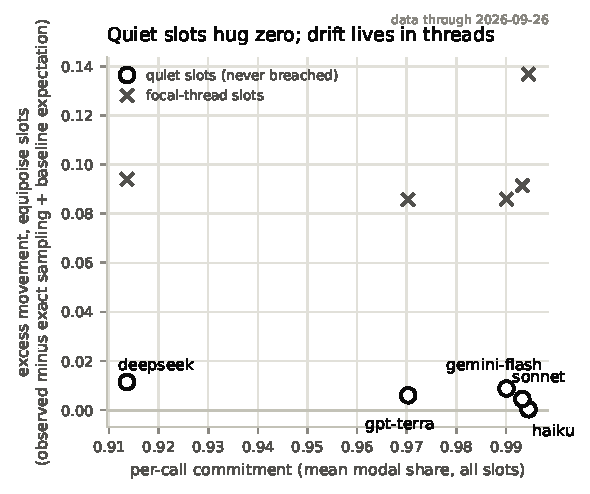
\includegraphics[width=0.9\columnwidth]{f4_phenotype_grid.pdf}
\caption{Phenotype grid. Per-call commitment (mean modal share of
a slot-day's ten samples) against excess movement on equipoise
slots (observed mean TVD minus the exact expectation with probe
sampling and $n{=}20$ baseline noise both charged). Circles are
never-breached slots, crosses are breached threads. Quiet slots hug
zero on every model; the drift lives in the threads.}
\label{fig:f4}
\end{figure}

The phenotypes are therefore two axes that do not reduce to each
other: how a model answers (per-call commitment) and how it moves
when it moves (thread morphology). The two Claude models and gpt
are commit-and-flip: near-deterministic per call (modal share 0.97
to 0.995), threads that are discrete oscillations with exact state
recurrence, every one of their ten repeat threads unidirectional.
The haiku thread is commit-and-flip at week scale: a
seven-observed-day rest, a sixteen-day away dwell, and a return to
a vector it had produced four weeks earlier. Deepseek is honest
noise with wander: the widest per-call spread in the roster (modal
share 0.91), quiet slots fully explained by sampling arithmetic
(excess $+0.011$), and the record's only mixed-direction threads,
three of its six, breaching toward two or three different options
from genuinely split baselines. Its other three threads are as
discrete and unidirectional as the Claude pair, so the wander is a
thread property that this vendor alone exhibits. Gemini sat
near-frozen through its 46 probe days: two transient breaches on
two different items and nothing held. Per-call determinism is not
temporal stability, and the most confident-looking style is the
least snapshot-auditable.

Format rides along as an independent observable. On the
vulnerability-gating item, answer state and response format flip in
lockstep: 567 of 580 rows are either a terse 9-character A or a
687-to-1,421-character reasoned D\rows. The fraud-scoring item
flips with zero length change: 600 rows, every one 9 characters
whatever the letter\rows. Format is a serving-state signal the
parsed-letter statistic only sees when the letter moves; it is
captured per row and reported descriptively.

\section{What the instrument got wrong}
\label{sec:wrong}

The CFP asks for honest failure. Seven items, each a dated commit
in the public record, each load-bearing for someone building the
same thing.

\begin{enumerate}
\item[(a)] The false-alarm arithmetic was wrong first. Working
  analysis estimated 3.4 chance breaches per day by treating p99
  as an exact exceedance rate; on a discrete statistic at $K{=}10$
  it is not. Exact enumeration corrected it to 1.64 (smoothed
  truth) and 0.05 (empirical truth); the correction is the citable
  number, and it moved to 1.65 when one slot was re-baselined.
\item[(b)] A sensitivity upgrade was approved, built, and declined
  the same day. $K{=}30$ narrows bands from roughly 0.40 to 0.267
  to 0.317; the between-day variance the bands never modeled sits
  at p99 0.30 on quiet equipoise slots at the freeze, above the
  proposed bands. At the freeze exceedance rates, shipping it would
  have manufactured 0.7 to 1.5 false alarms per day from quiet
  equipoise slots alone. The reason is measured, not assumed: the
  equipoise mean daily TVD decomposes into a sampling term and a
  between-day excess, and a $K{=}30$ projection shrinks the mean to
  0.71 of its $K{=}10$ value, not the 0.58 that square-root scaling
  predicts, because the excess does not shrink with $K$.
\item[(c)] The frozen baseline can be the anomaly. 82 of 115
  equipoise slots were unanimous at baseline, on items designed to
  split. For those slots the monitor may have enshrined an
  excursion as the reference and then alarmed on movement toward
  designed behavior; three of the 82 breached. The instrument
  therefore says ``changed,'' never ``degraded''; the sign of change
  is not identified.
\item[(d)] EVENT certifies minutes, not the roughly twenty the
  design assumed. Measured item-level probe-to-rerun gaps run 0.34
  to 10.15 minutes\rows. The label was demoted in the analysis
  rather than defended.
\item[(e)] The first version of this paper's phenotype figure
  repeated the baseline error in miniature. Its expected-movement
  term treated the frozen $n{=}20$ baseline as exact, which charges
  the widest-distribution vendor for its own sampling spread, and
  the figure misread honest noise as drift. The corrected
  expectation propagates baseline noise exactly; mistake and
  correction are same-day dated commits.
\item[(f)] The breach comparison ran in floating point on
  quantities that are exact rationals, and the summation path
  decided real verdicts. A bit-faithful census (committed script)
  finds 10 of the 75 entries fired on exact at-band equalities the
  float path read as strictly above, from both sides of the
  comparison; zero breaches were missed; one item verdict flipped
  at the rerun gate (an EVENT that is a TRANSIENT under exact
  arithmetic); six day verdicts change, five TRANSIENT to CLEAN and
  the record's only UNSTABLE to CLEAN. The verdict log stands as
  recorded; every headline claim survives both semantics (65
  entries on 16 slots, all equipoise); the false-breach null moves
  in step (1.65 to 1.55); the instrument moves to exact integer
  comparison after submission, on a dated schedule.
\item[(g)] The monitor is only as continuous as its operator.
  Twenty-one model-days in 56 returned no probe: three to exhausted
  API credit, two to a credential rotation, ten to one vendor's
  HTTP 503 responses, five to a local network outage on a single
  day. None is a behavioral observation, all are in the log, and a
  production deployment needs the same alarm on the monitor's own
  availability that it puts on the model.
\end{enumerate}

\section{Operational guidance}

For a team running judgment-layer automation on a frontier API,
the numbers above convert to practice.

\textbf{Split the bank by class and band accordingly.} Decisive
items are near-noiseless: in 11,057 slot-days the maximum TVD was
0.30, seen twice, and 0.20 was exceeded seven times. A decisive
band of 0.30 would never have fired in 56 days; 0.25 would have
fired twice. Either is a large gain over the deployed 0.40, and
monitoring there is essentially free sensitivity, provided the
pre-registered rollback (revert if the tightened class produces
three entries in fourteen days) rides along. Equipoise bands cannot
narrow at $K{=}10$: between-day spread does not shrink with $K$
(item b), so they stay at 0.40 or above and their alarms are read
as regime signals, not degradation.

\textbf{Treat snapshot evaluation as day-certification.} A passed
eval certifies the day it ran. Period assurance requires a monitor
in the loop, and the monitor defines the compensating control:
route flagged periods to secondary review, gate automated decisions
qualified against prior behavior, and write the observable into
vendor contracts (distribution stability on a pinned bank), not the
cause, which no customer can observe.

\textbf{Re-baseline without discarding.} When a monitored slot
settles into a new state and the alarm channel turns into a daily
repeat of the same event, do not choose between the old reference
and the new one; keep both. Move the alarm to the new reference,
preserve the original in the same record, and pre-register the
return criterion before any new-regime data accrues. The first use
of this pattern ran its full loop inside the record: rule fired,
re-baseline the same day, return detected on post-rebaseline day
10, pre-registered revision the same day as detection, seven more
return visits after that (Section~\ref{sec:loop}). A bare
re-baseline would have converted a slow alternator into a permanent
misclassification; the preserved reference is the difference
between the two.

\textbf{Pin by served identity, not by request string.} The
request id is an input; the identity that answers is an
observation, and they can diverge without any request failing.
When the deepseek flash tier was renamed mid-study, the pinned id
kept serving as a silent alias, and only the response-side echo
distinguished the qualified model from whatever now answered to its
name. Record the echo on every row, halt on divergence, and treat
the halt as an event: that converted an invisible reroute into a
dated detection at first contact.

\textbf{Budget for the monitor's own gaps.} Credit, credentials,
vendor availability, and the operator's network each took days out
of this record (item g). Alarm on a missing probe the way you alarm
on a breach; a quiet log and an absent log look the same from a
distance.

\textbf{Know what the tool cannot do.} Detection tells you when to
stop trusting your own automation. It does not tell you whom to
blame, and procurement or contract language that assumes
attribution from outside the API is writing a check the
measurement cannot cash.

\section{Related work}

Log-probability and token-level API change
detection~\cite{chauvin-a,chauvin-b} targets the same problem with
instruments that require persistence: multi-day filters and one-way
changepoints. The oscillation class documented here is discarded by
those designs by construction; a state that reverts within days
never survives a four-day persistence filter. The instruments are
complementary, and the reversible class needed one that keeps it.
Daily and weekly periodicity in LLM performance~\cite{tschisgale}
is the continuous cousin of the discrete recurrence here.
Longitudinal behavioral change on major APIs is established at
month scale~\cite{chen}; this work moves the resolution to days and
adds exact state recurrence. The attribution ceiling is structural,
not a limitation of effort: black-box access does not support
causal attribution of serving-stack change~\cite{casper}, and
software-only verification of served models remains
brittle~\cite{cai}. Boundary-item drift sensing predates LLMs:
margin-density drift detection placed its sensors at the decision
boundary~\cite{md3}, the same design choice the equipoise class
makes here. Vendor-side ground truth that serving changes ship,
stick per-user, and evade vendor evals comes from a published
postmortem~\cite{anthropic-postmortem}; the numerics mechanism for
silent behavioral variation is documented
in~\cite{thinking-machines}.

\section{Limitations and reproducibility}

One bank, five models, one scaffold, 56 days. The phenotypes are
observed styles, not vendor properties. Slots within a model-day
share a scaffold; day-level counts are overdispersed and the
per-slot recurrence statistics carry the independence caveat stated
in Section~\ref{sec:null}. The detection floor at $K{=}10$ is a
four-to-five-of-ten answer shift, so sub-floor movement is
invisible and decisive-class stability is bounded, not proven. The
strict inequality at the band is load-bearing, and its float
implementation decided ten at-band entries (item f); every reported
number carries its exact-arithmetic companion from the committed
census. One arm's behavioral record ends on day 39 by its own
tripwire, and another arm's availability failed for the last eight
days of the window; the per-model day counts are 53, 53, 52, 46,
and 39. The per-call rows that carry response text, and therefore
the format and covariate constancy numbers marked \rows, are
retained but not published; everything else is. Cost and cadence
are modest by design; the instrument trades sensitivity for a
false-alarm budget an operator can actually staff.

The full instrument is reproducible: item bank, baselines, bands,
seeds, verdict log, derived daily counts, analysis scripts, and
every correction cited above as dated history. The artifact is
public; the link is withheld from this submission for blind review
and supplied on acceptance.

\bibliographystyle{IEEEtran}
\bibliography{refs}

\end{document}
